\section{Electrical reproduction of sound}

\bi
\i A basic understanding of electricity and magnetism is 
needed to describe the functioning of musical recording 
and reproduction equipment.

\i Here, we briefly describe electrical circuits (voltage, current,
resistance, power, $\cdots$) and also Faraday's law of induction, 
which underlies the operation of microphones and loudspeakers.

\ei

%%%%%%%%%%%%%%%%%%%%%%%%%%%%%%%%%%%%%%%%%%%%%%%%%%%%%%%%%%%
\subsection{Basic electricity}

\bi

\i When a voltage source (such as a battery) is connected to a 
load (such as a flashlight bulb) via a closed path (called a
circuit), an electrical current flows.

\i The voltage is denoted by $V$ and is measured in volts (V).
The load has a {\em resistance}, which is denoted by $R$ and 
measured in Ohm ($\Omega$).
The current is denoted by $I$ and is measured in Ampere or 
Amp (A).

\i For certain materials, $V$, $I$, and $R$ are related by 
%
\be
R=V/I\quad{\rm or,\ equivalently,}\quad 
V= IR
\ee
%
This is called {\em Ohm's law of electricity}, not to be confused
with Ohm's law of hearing, even though it's the same guy.

\i For a battery, which has a {\em polarity} ($+$ and 
$-$ terminals), the current $I$ flows in only one direction, 
which we take to be from the $+$ terminal of the battery 
to the $-$ terminal.
This is called a {\em direct current} (DC) circuit.
(See the left-hand panel of Figure~\ref{f:circuits_DC_AC}.)
%
\begin{figure}[htbp]
\begin{center}
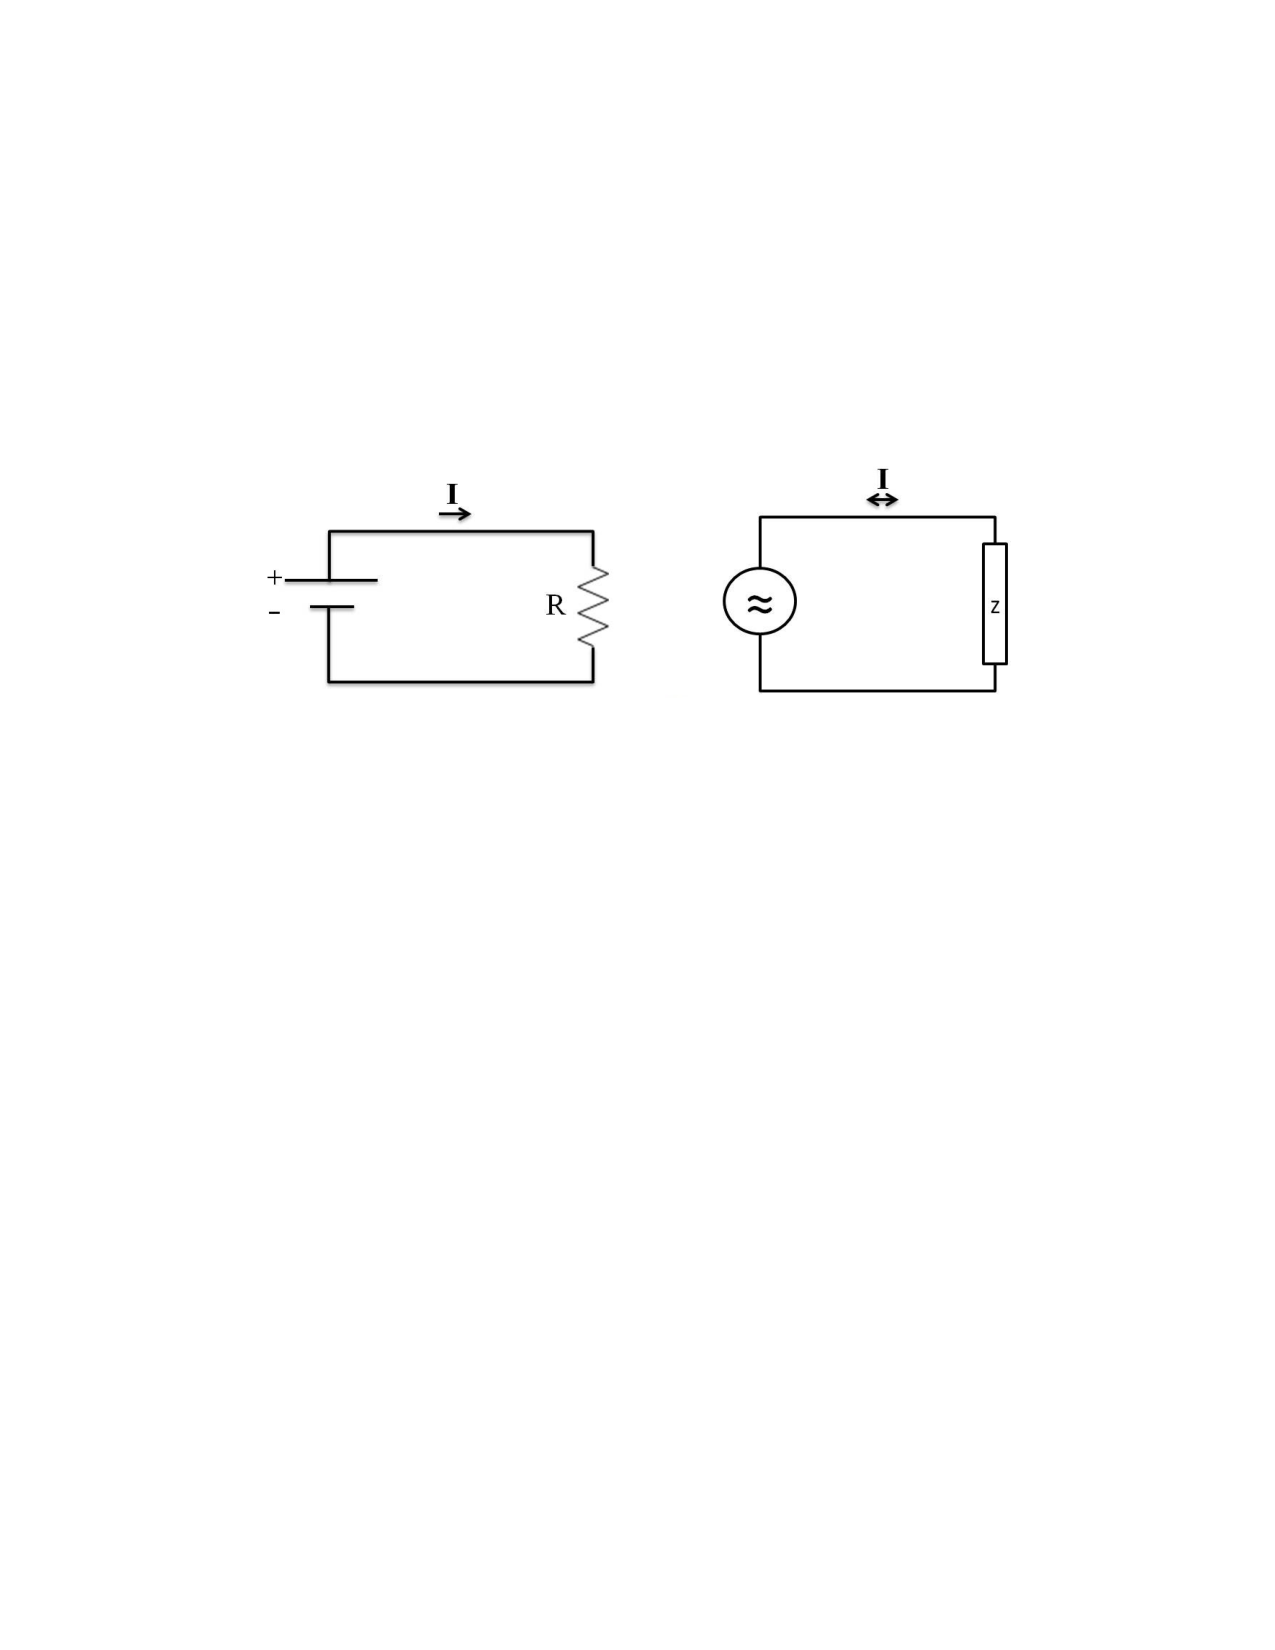
\includegraphics[width=0.75\textwidth]{circuits_DC_AC}
\caption{Left: Direct current (DC) circuit, consisting
of a voltage source $V$ and load having resistance $R$.
Right: Alternating current (AC) circuit, consisting of
a voltage source $V$ and load having impedance $Z$.
For a DC circuit, the current $I$ flows in only one direction.
For an AC circuit, the current $I$ flows alternately clockwise and
counterclockwise.
(Figures from ``PHYS 1406: Physics of Sound \& Music" 
Course Guide by Prof.~Borst.)}
\label{f:circuits_DC_AC}
\end{center}
\end{figure}

\i For a household wall outlet, the voltage $V$ alternates
sinusoidally with time, producing a current $I$ that 
also alternates sinusoidally, traveling both clockwise and 
counterclockwise around the circuit.
Such a circuit is called an {\em alternating current} (AC) circuit.
(See the right-hand panel of Figure~\ref{f:circuits_DC_AC}.)

\i For AC circuits, there is a relation 
%
\be
V = I Z
\ee
%
which is similar to Ohm's law, but it involves the {\em impedance}
$Z$ of the load.

\i Impedance is basically a generalization of resistance, which holds
for electrical devices such as {\em capacitors} (basically,
closely-spaced metal plates, which store electric charge) and {\em
inductors} (basically, coils of wire, which store electric currents).

\i The product 
%
\be
P = VI
\ee
%
is the electrical {\em power} associated with a circuit.
(For AC circuits, the formula is slightly more complicated than this,
but we don't need to know the details.)
Power is measured in Watt (W), such as that for a 100-W light bulb.

\i \exer
Using Ohm's law $V=IR$, show that
%
\be
P=VI=I^2 R = V^2/R
\ee

\i In general, power is the rate at which {\em work} (or {\em energy})
is  being done. 
If we denote the work (or energy) by $W$ done in a time interval
$\Delta t$, then
%
\be
P = W/\Delta t
\quad{\rm or,\ equivalently,}\quad
W = P\,\Delta t
\ee
%
Work (or energy) is measured in Joules (J), where 1~Watt =
1~Joule/sec.

\i Application: A kilowatt-hour (kWh) is a convenient unit of 
energy that you will see on electric bills.
In terms of Joules
%
\be
1~{\rm kWh}
= 1~{\rm kW}\times 1~{\rm hr}
= 1000~{\rm W} \times 3600~{\rm s}
= 1000~{\rm J/s} \times 3600~{\rm s}
= 3.6\times 10^6~{\rm J}
\ee

\i \exer 
Suppose that you paid \$100 for last month's electrical bill
at cost of \$0.13 per kWh.
(a) How many kWh did you use? 
(b) What was the average power consumption (in Watt) over 
the month (assume 30~days).

\i \ans

(a) 
\be 
W=\$100 \div \$0.13/{\rm kWh} = 769~{\rm kWh}
\ee 

(b)
\be
P = \frac{W}{\Delta t} 
= \frac{769~{\rm kWh}}{30\times 24~{\rm h}} 
= 1.1~{\rm kW} 
= 1,100~{\rm W}
\ee

This is equivalent to using eleven 100-W light bulbs 
continuously for a month.
 
\ei

%
%%%%%%%%%%%%%%%%%%%%%%%%%%%%%%%%%%%%%%%%%%%%%%%%%%%%%%%%%%%
\subsection{Faraday's law}

%
\begin{figure}[htbp]
\begin{center}
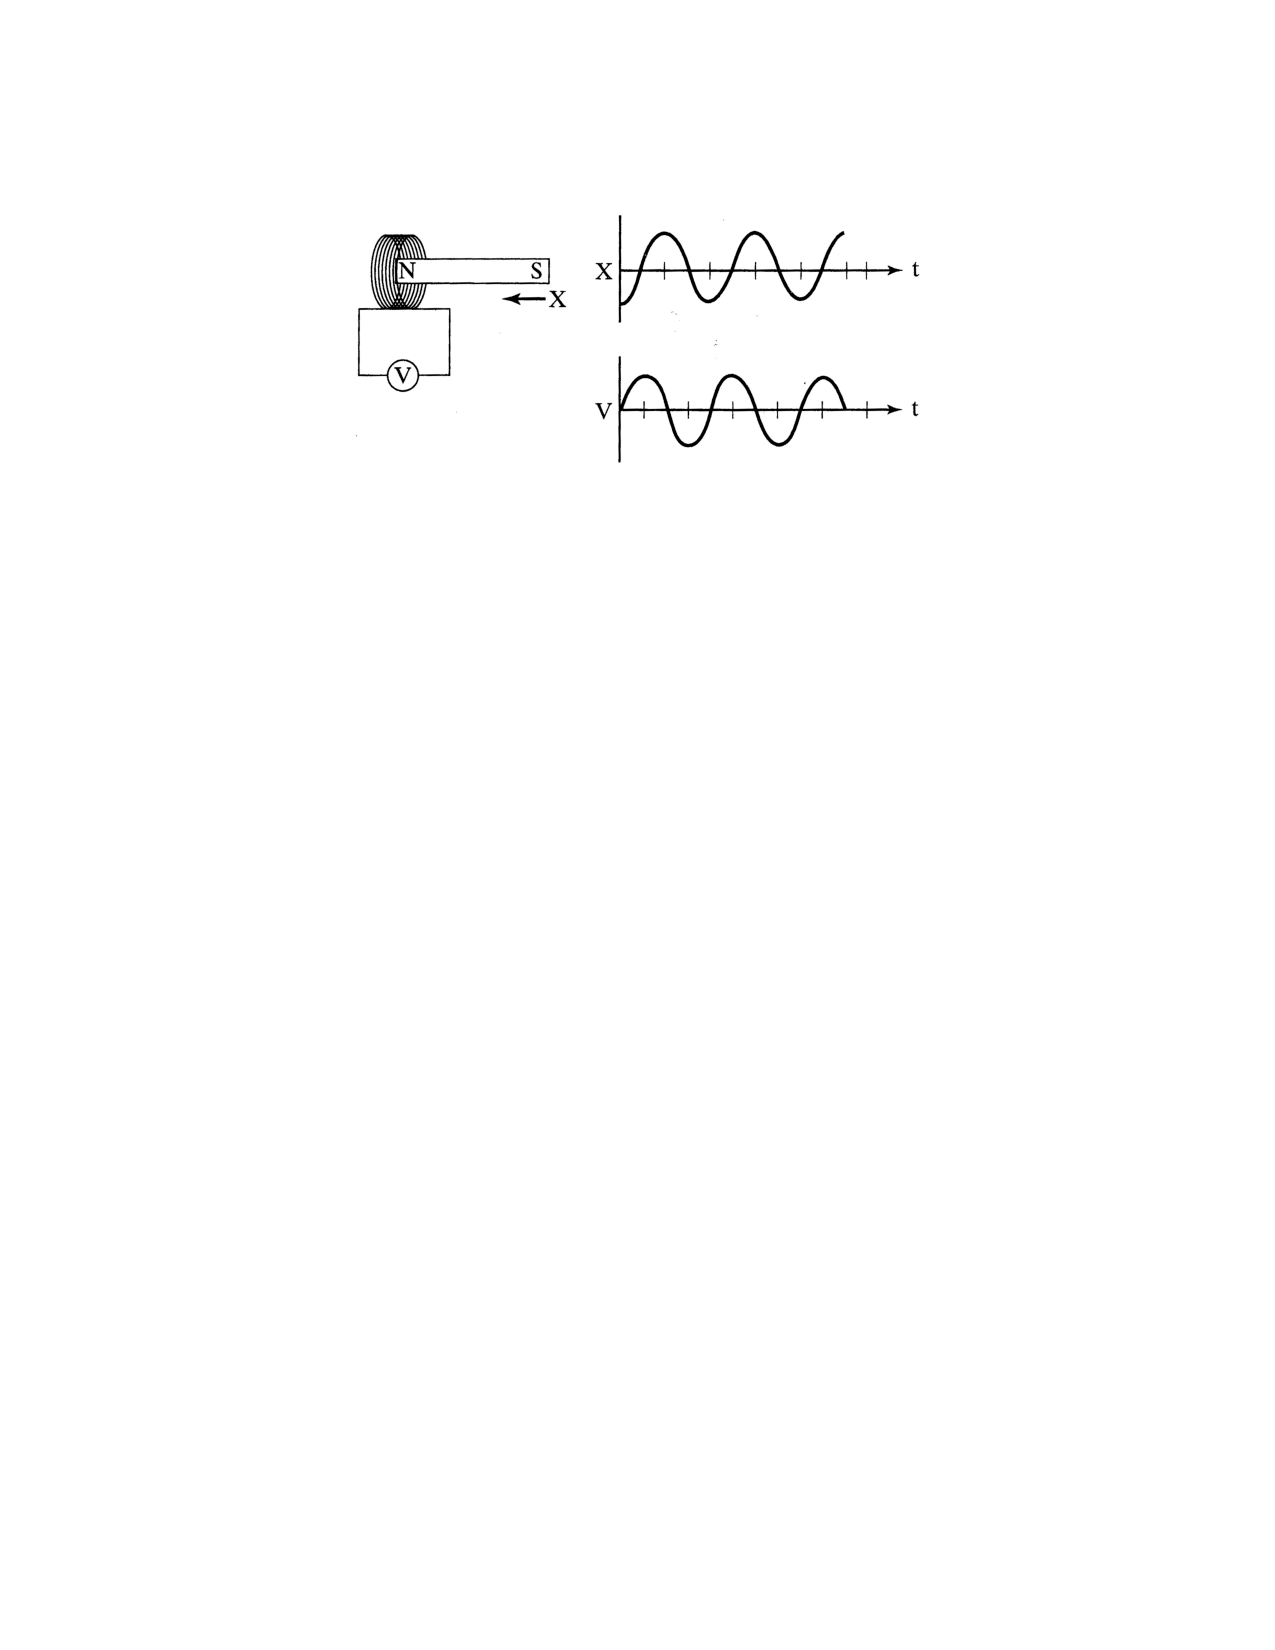
\includegraphics[width=0.6\textwidth]{faraday}
\caption{Illustration of Faraday's law.
As a magnetic moves back and forth ($X$ vs $t$) in the vicinty 
of a coil of wire, an alternating voltage ($V$ vs $t$) is induced
in the coil.
(Figure from ``Physics of Sound," by Berg and Stork.)} 
\label{f:faraday}
\end{center}
\end{figure}
%

%%%%%%%%%%%%%%%%%%%%%%%%%%%%%%%%%%%%%%%%%%%%%%%%%%%%%%%%%%%
\subsection{Microphones and loudspeakers}
%
\begin{figure}[htbp]
\begin{center}
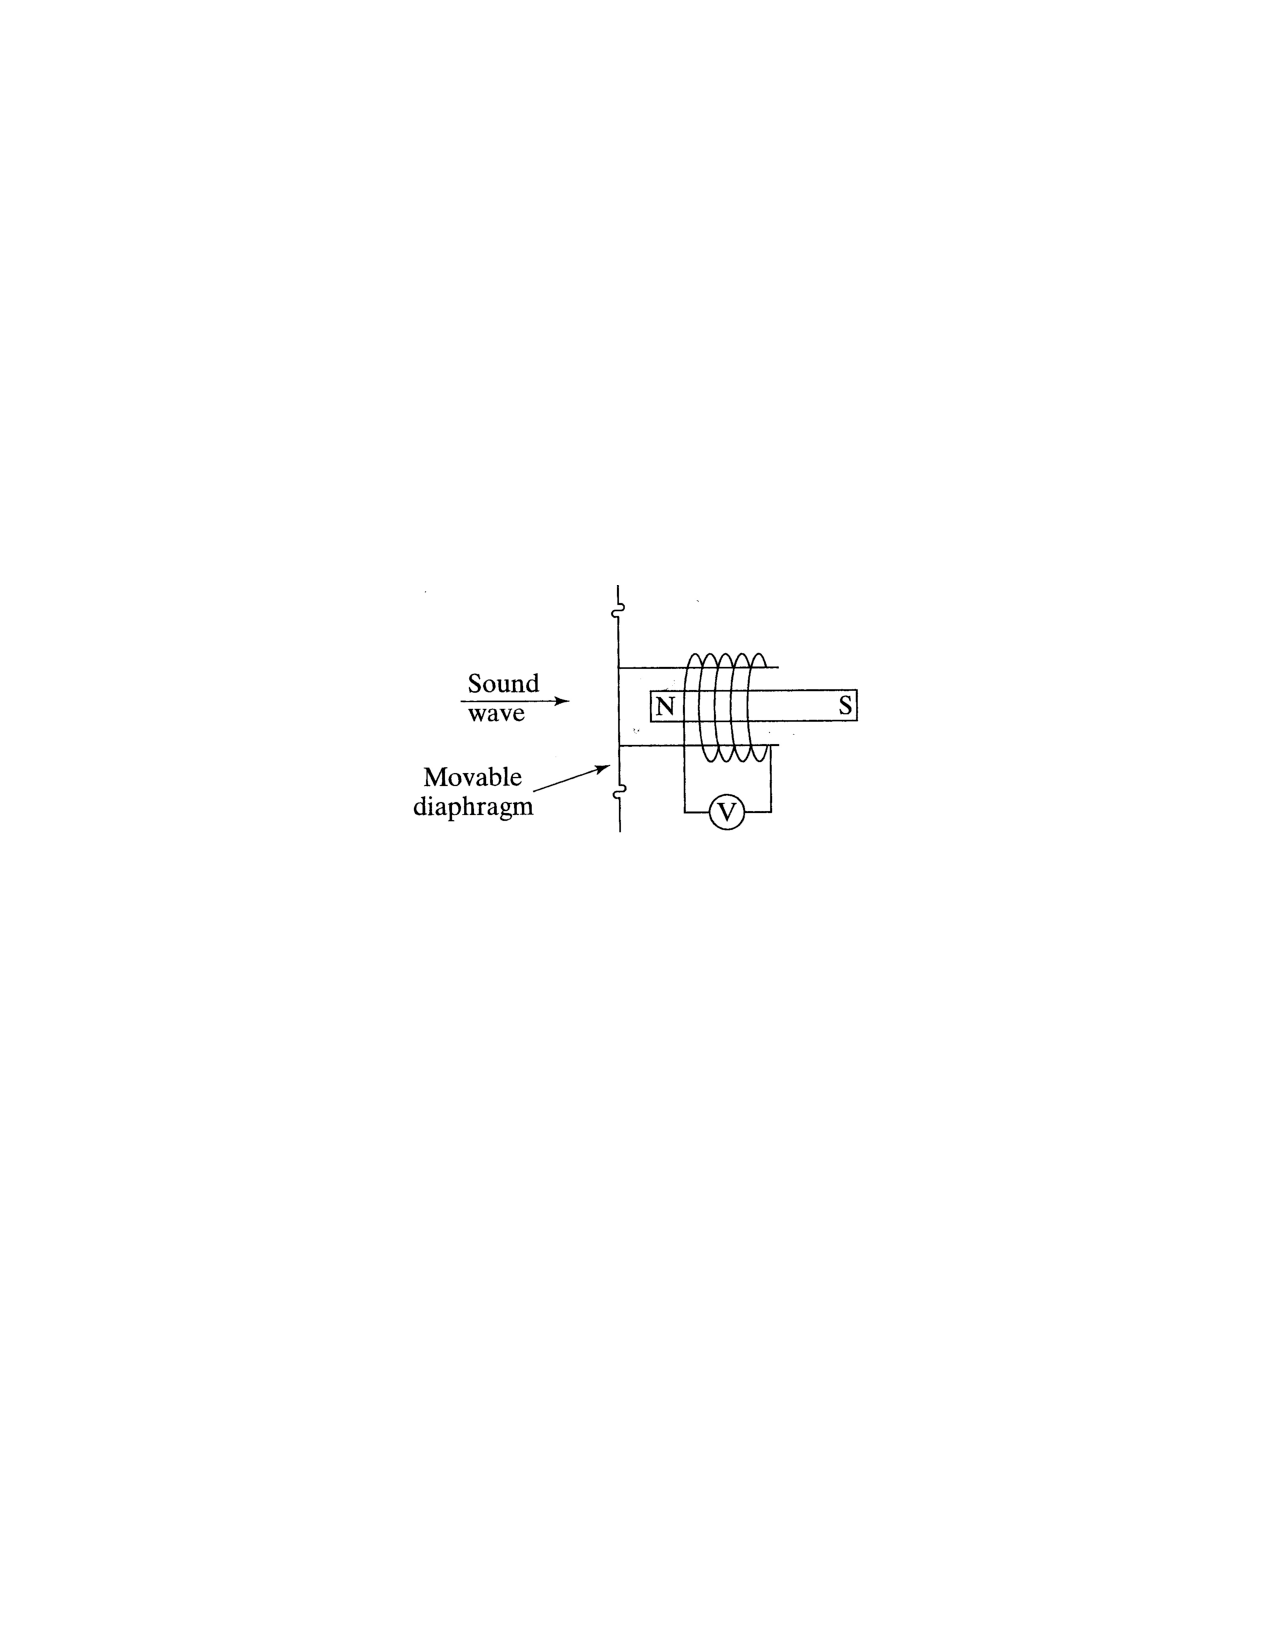
\includegraphics[width=0.5\textwidth]{microphone}
\caption{Schematic diagram of a dynamics microphone.
The pressure deviation associated with a sound wave
pushes back and forth on the diaphragm of the microphone.
A coil of wire, which is attached to the diaphragm, thus
moves in the presence of a magnetic field.
The changing magnetic flux through the coil induces a voltage $V$ in
the coil which follows the fluctuations of the sound wave.
(Figure from ``Physics of Sound," by Berg and Stork.)} 
\label{f:microphone}
\end{center}
\end{figure}
%
%
\begin{figure}[htbp]
\begin{center}
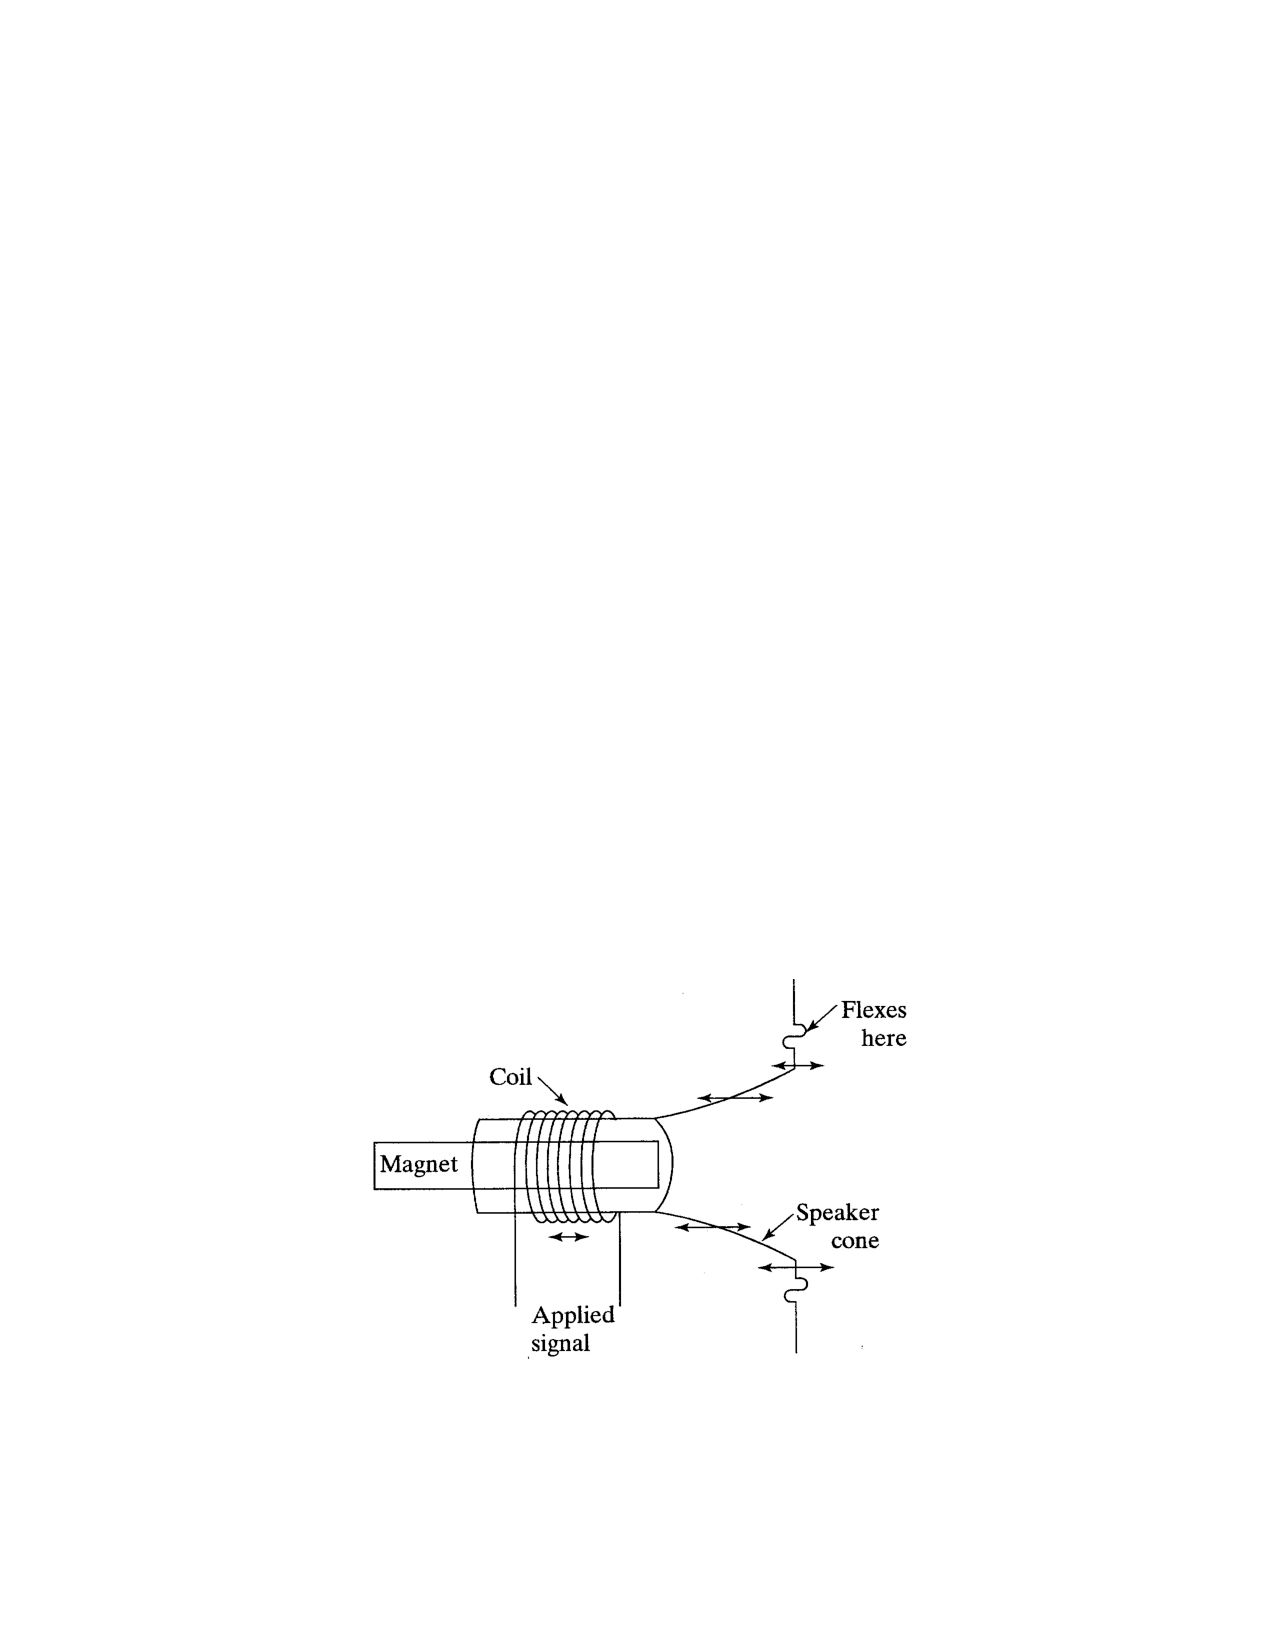
\includegraphics[width=0.5\textwidth]{loudspeaker}
\caption{An electrical signal applied to the coil 
creates a magnetic field that interacts with that of the
permanent magnetic.
The speaker cone, which is attached to the coil, 
moves back-and-forth in repsonse to this interaction,
thus producing a sound wave. 
(Figure from ``Physics of Sound," by Berg and Stork.)} 
\label{f:loudspeaker}
\end{center}
\end{figure}
%
%
\begin{figure}[htbp]
\begin{center}
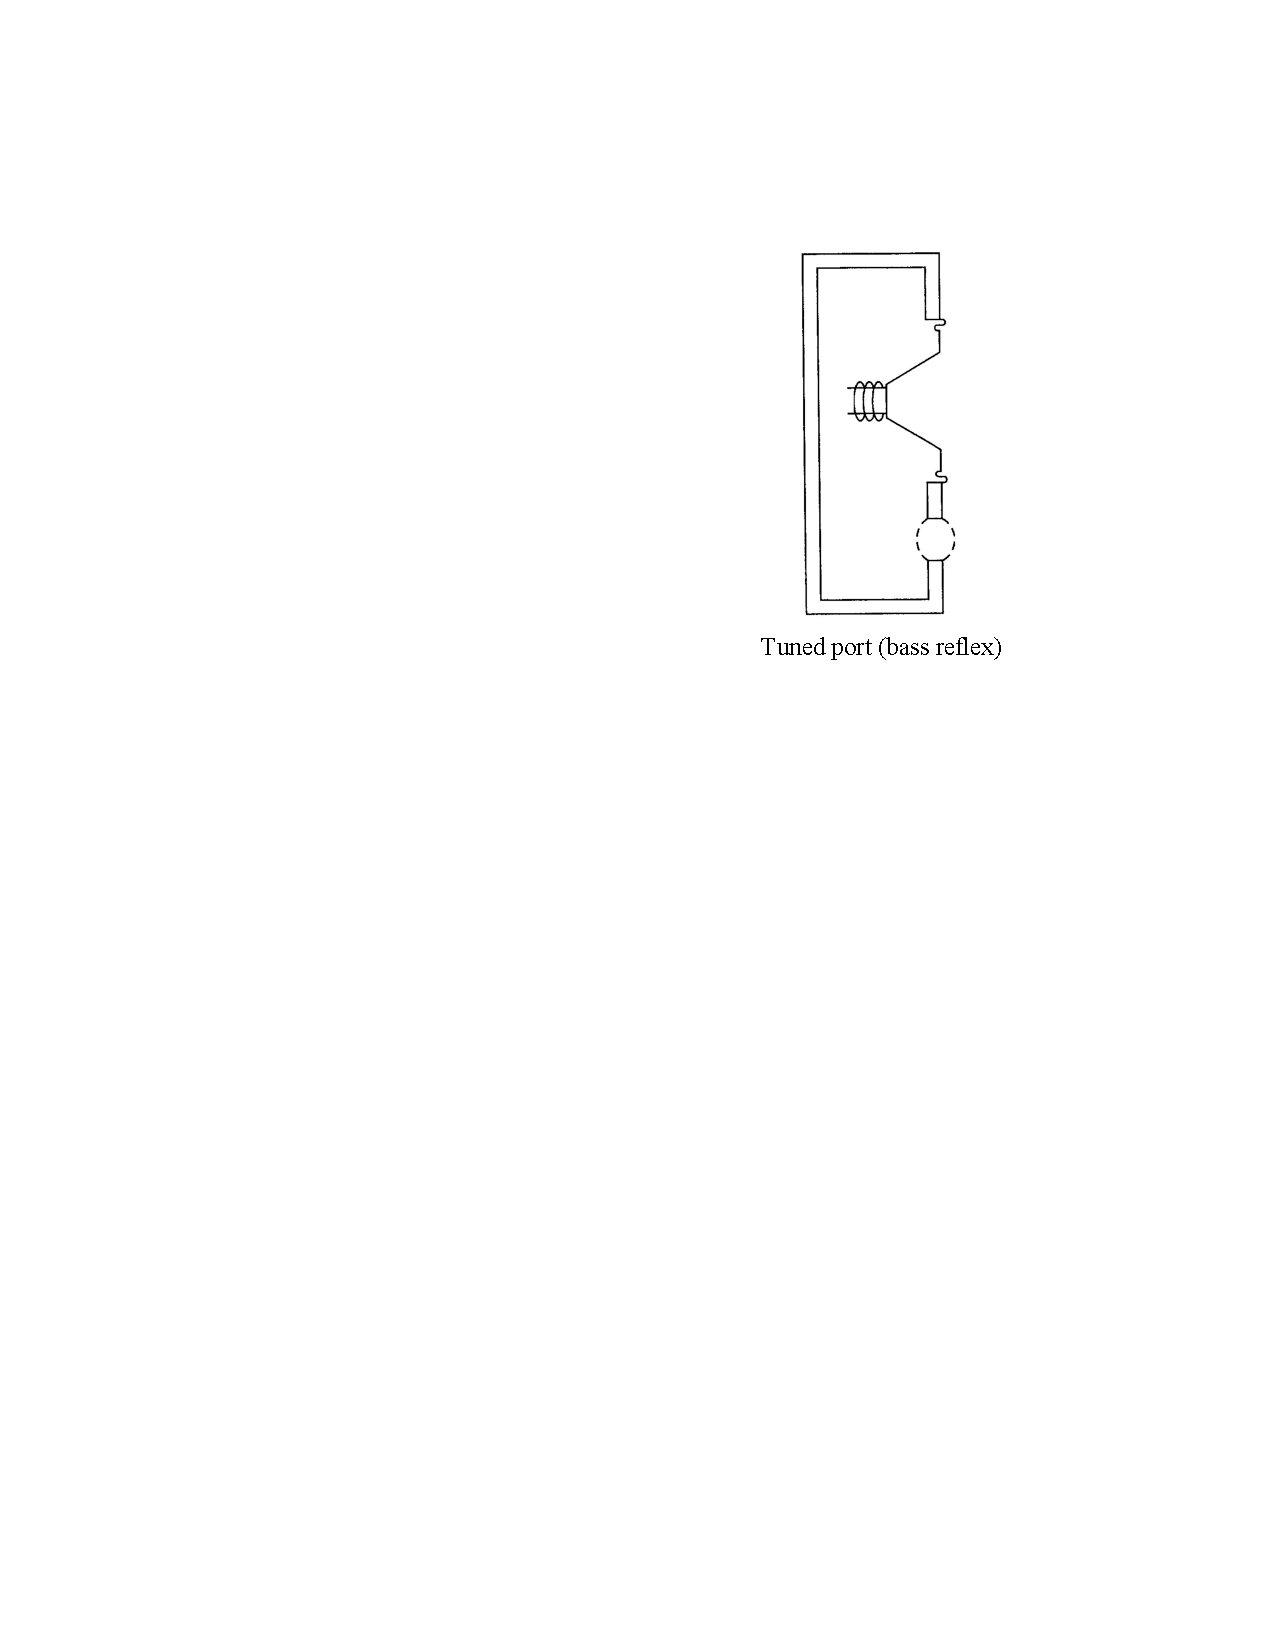
\includegraphics[height=0.4\textwidth]{loudspeaker_tunedport}
\hspace{0.2in}
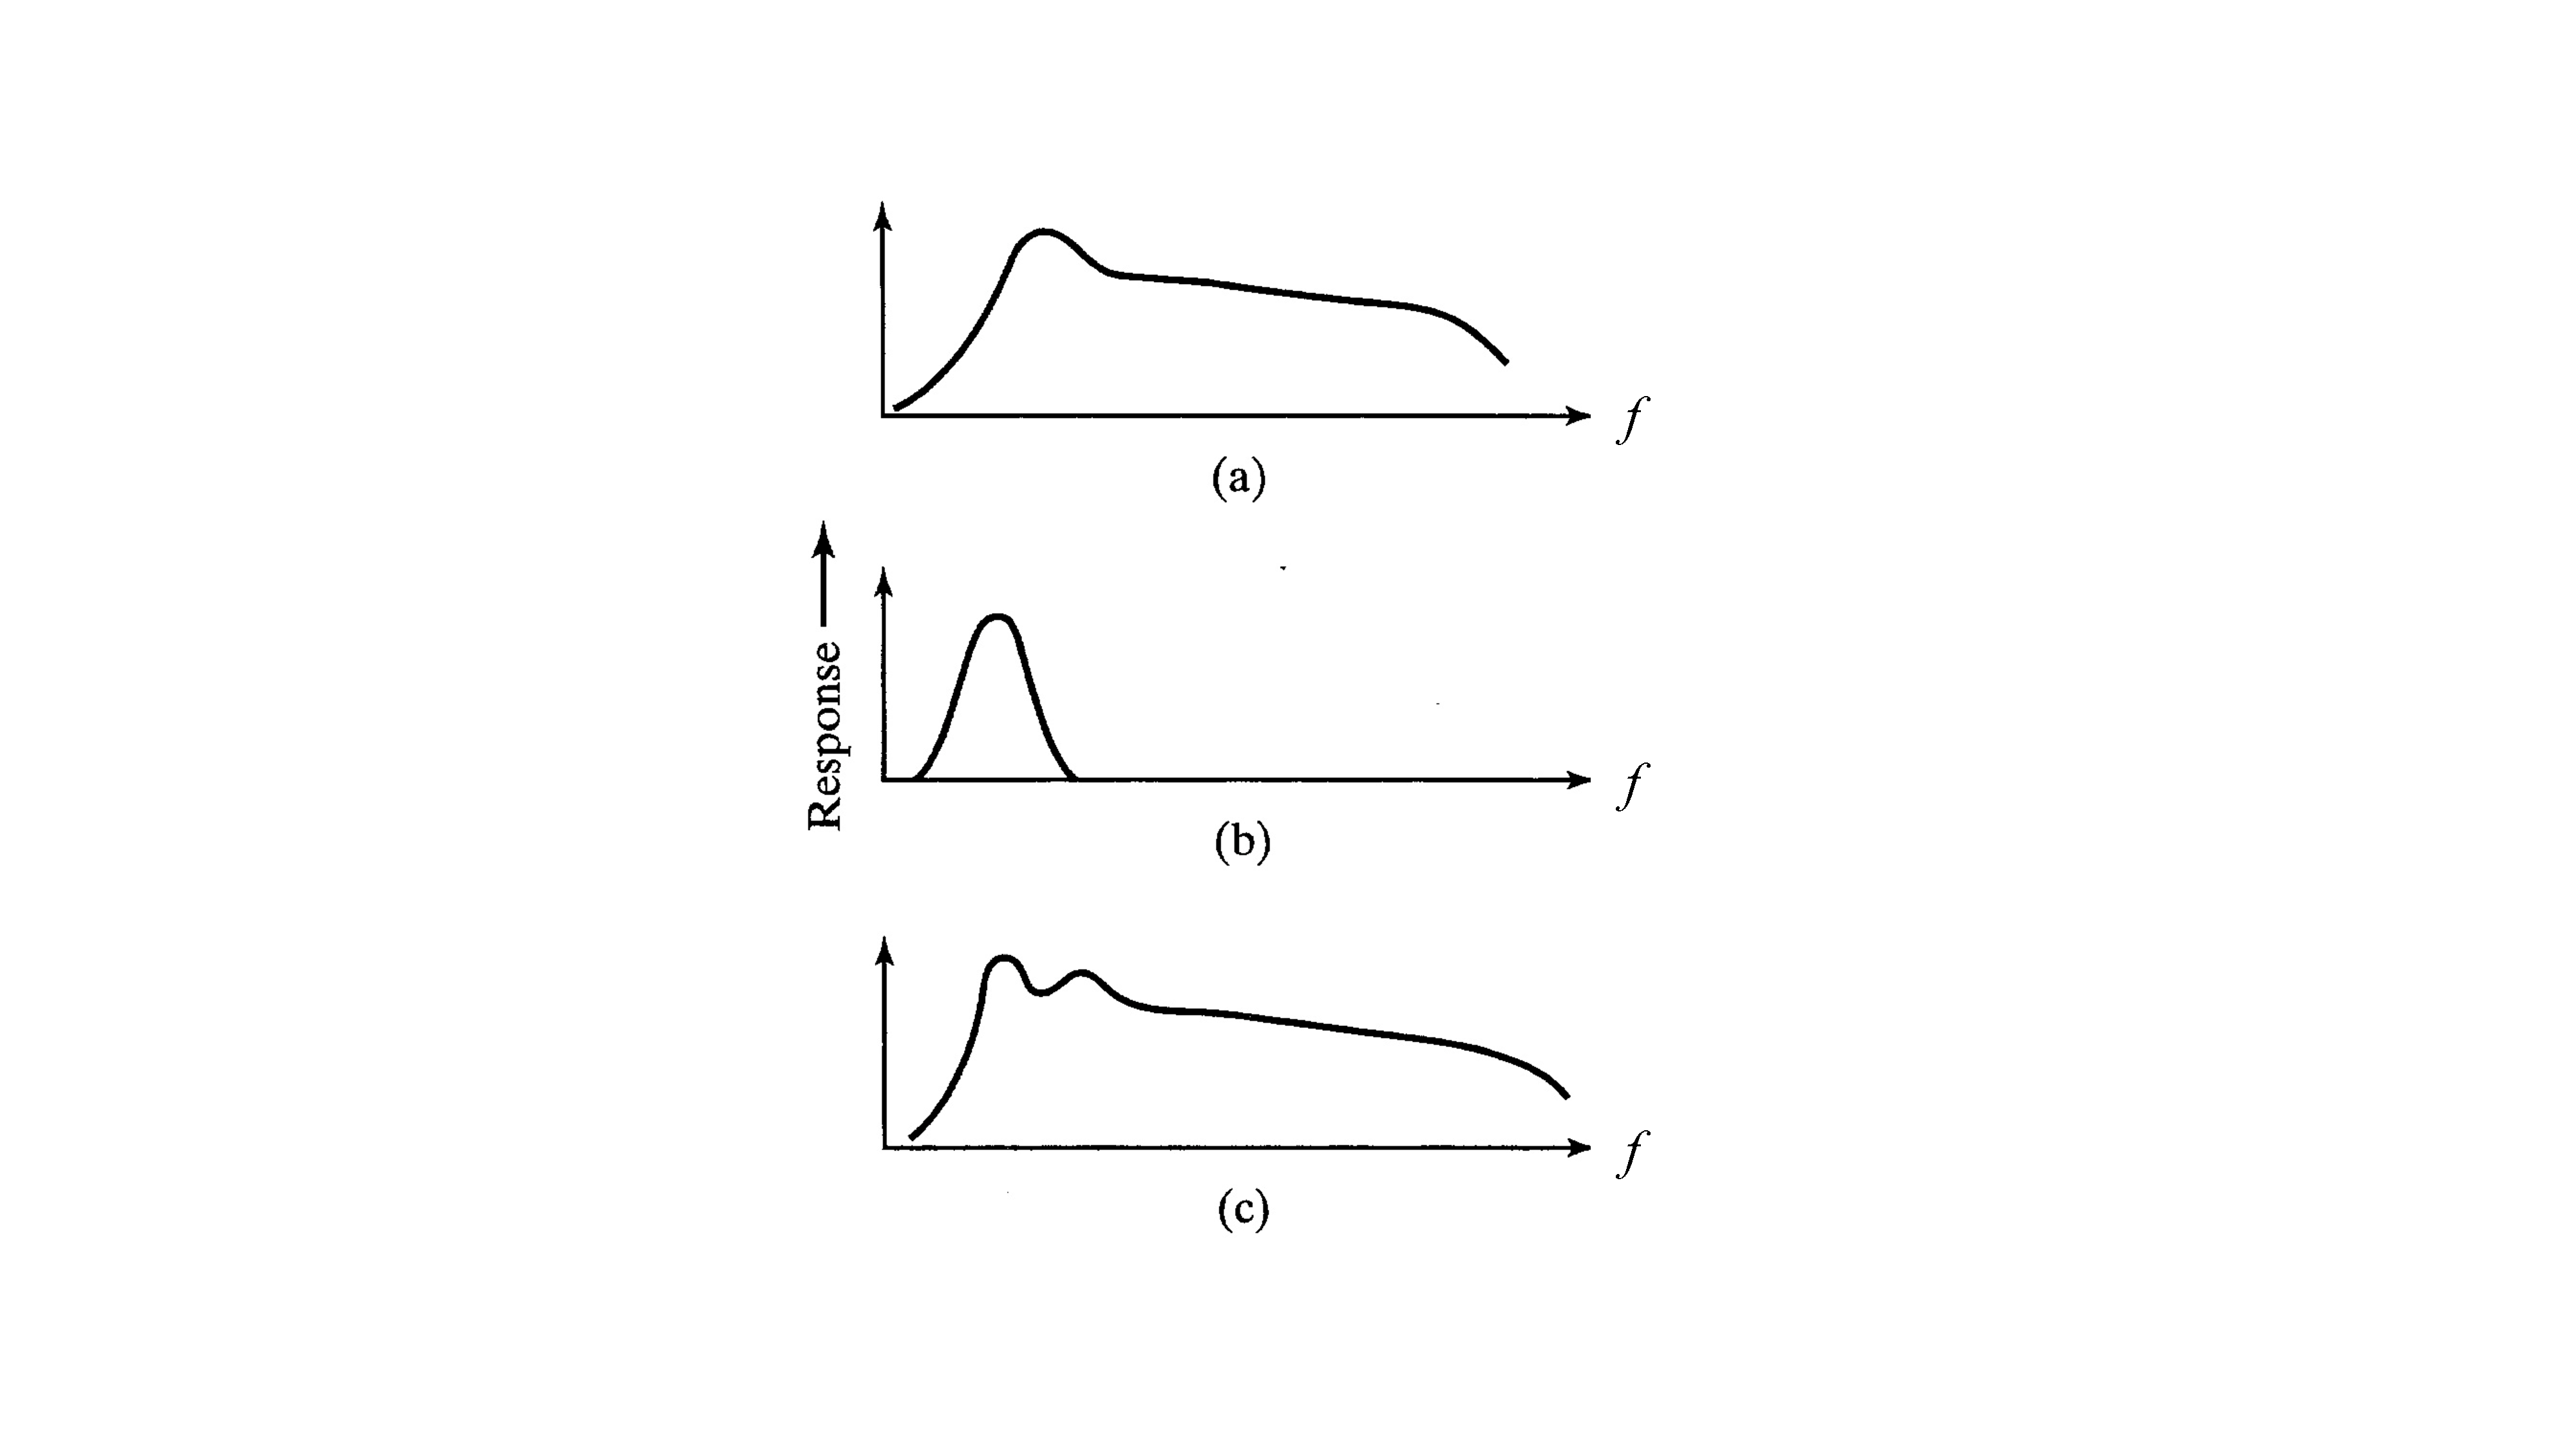
\includegraphics[height=0.4\textwidth]{loudspeaker_tunedport_response}
\caption{Acoustic-suspension and tuned-port loudspeakers (left, middle); 
frequency response curves (right).
(a) Frequency repsonse for an acoustic-suspension loudspeaker.
(b) Frequency response of an empty box with a hole (tuned port), 
which acts like a Helmholtz resonator.
(c) Combined frequency response for a tuned-port loudspeaker.
(Figures from ``Physics of Sound," by Berg and Stork.)} 
\label{f:loudspeaker_tunedport}
\end{center}
\end{figure}
%

